\chapter{Теорема Лиувилля и гамильтонов поток}

\lectureoverview{Уравнения Гамильтона делают больше, чем просто переупаковывают уравнения движения. Они задают поле скоростей в фазовом пространстве, дивергенция которого равна нулю. Это простое взаимное сокращение и есть теорема Лиувилля: гамильтонова эволюция сохраняет фазовый объем. Мы придем к ней в том порядке, в котором становится виден ее смысл---сначала сохранение энергии, затем поверхности постоянной энергии, затем жидкость возможных начальных условий и, наконец, контраст между потоком, сохраняющим объем, и диссипативным стоком. Тот же язык естественным образом приводит к скобкам Пуассона.}

\section{Зачем нужна еще одна формулировка механики?}

Теорема, которая нам нужна, — это непрерывный классический аналог обратимых диаграмм состояний, введенных в начале курса. В обратимом дискретном законе в каждое состояние входит одна стрелка и из него выходит одна стрелка. Настоящего состояния достаточно, чтобы определить и следующее состояние, и предыдущее. Плохой закон направляет много состояний в один сток: будущее может быть определено, но прошлое уже нельзя восстановить.

Теорема Лиувилля говорит, во что превращается это различие, когда множество состояний представляет собой непрерывное фазовое пространство. Фразой, заменяющей одну входящую и одну выходящую стрелку, будет \emph{сколько потока втекает, столько и вытекает}. Однако прежде чем придать этой фразе математический смысл, нам нужно восстановить поток из уравнений Гамильтона.

При этом возникает историческая загадка. Гамильтон, Якоби, Лагранж и Пуассон построили сложные и прекрасные формы классической механики, не зная квантовой теории, в которой эти формы станут незаменимыми. У Ньютона была прямая цель: движение планет. Перед Лагранжем и Гамильтоном тоже стояли физические задачи, но они разрабатывали аналогии и структуры, далеко выходящие за пределы какой-либо одной орбиты. Стационарное действие в механике напоминало принципы наименьшего времени в оптике; движение лучей и движение частиц можно было выразить в параллельных математических формах. Они упрощали, перестраивали и объединяли уравнения, потому что сами структуры, казалось, содержали физику.

Теперь мы знаем, что это чутье оказалось необычайно плодотворным. С логической точки зрения многие черты классической механики можно понять как пределы квантовой механики. Исторически порядок был обратным: классические структуры были найдены сначала, и лишь гораздо позже прояснилось их более глубокое применение. Провокационная шутка, приписываемая Фейнману, подчеркивала это, противопоставляя математику, развиваемую из внутренних соображений, физике, ограниченной внешним партнером — физическим миром. Шутка — не аргумент, но различие полезно: формальная красота здесь важна, потому что природа снова и снова выбирает именно эти формальные структуры.

\begin{classroomqa}
  \audiencequestion{Было ли у Ньютона современное понятие кинетической энергии и откуда берет начало понятие энергии?
  \lecturetimestamp{00:04:24--00:05:50}}
  \lecturerresponse{Механика Ньютона была организована вокруг силы и движения, а не вокруг развитого общего принципа энергии. Точный исторический приоритет в этом обсуждении не устанавливается. Лейбницево \emph{vis viva},
  \(\sum_i m_i v_i^2\), было важным предшественником и равно удвоенной современной кинетической энергии. Позднейшие исследования теплоты сделали центральной проблему превращения теплоты в механическую работу. Ранние калорические теории рассматривали теплоту как сохраняющуюся субстанцию, поэтому современное представление о взаимопревращаемых формах энергии сложилось лишь постепенно.}
\end{classroomqa}

\section{Уравнения Гамильтона и сохранение энергии}

Пусть система имеет \(n\) канонических пар,
\begin{equation}
  (q_i,p_i),\qquad i=1,\ldots,n.
  \label{eq:l7-canonical-pairs}
\end{equation}
Каждой координате соответствует один импульс, и каждому импульсу — одна координата. Закон движения заключен в одной функции,
\begin{equation}
  H=H(q_1,\ldots,q_n,p_1,\ldots,p_n,t),
  \label{eq:l7-hamiltonian}
\end{equation}
а уравнения Гамильтона имеют вид
\begin{equation}
  \boxed{
  \dot q_i=\frac{\partial H}{\partial p_i},
  \qquad
  \dot p_i=-\frac{\partial H}{\partial q_i}.}
  \label{eq:l7-hamilton-equations}
\end{equation}
Знак является частью канонической структуры. В уравнении для \(q\) стоит плюс; в уравнении для \(p\) — минус.

\begin{figure}[htbp]
  \centering
  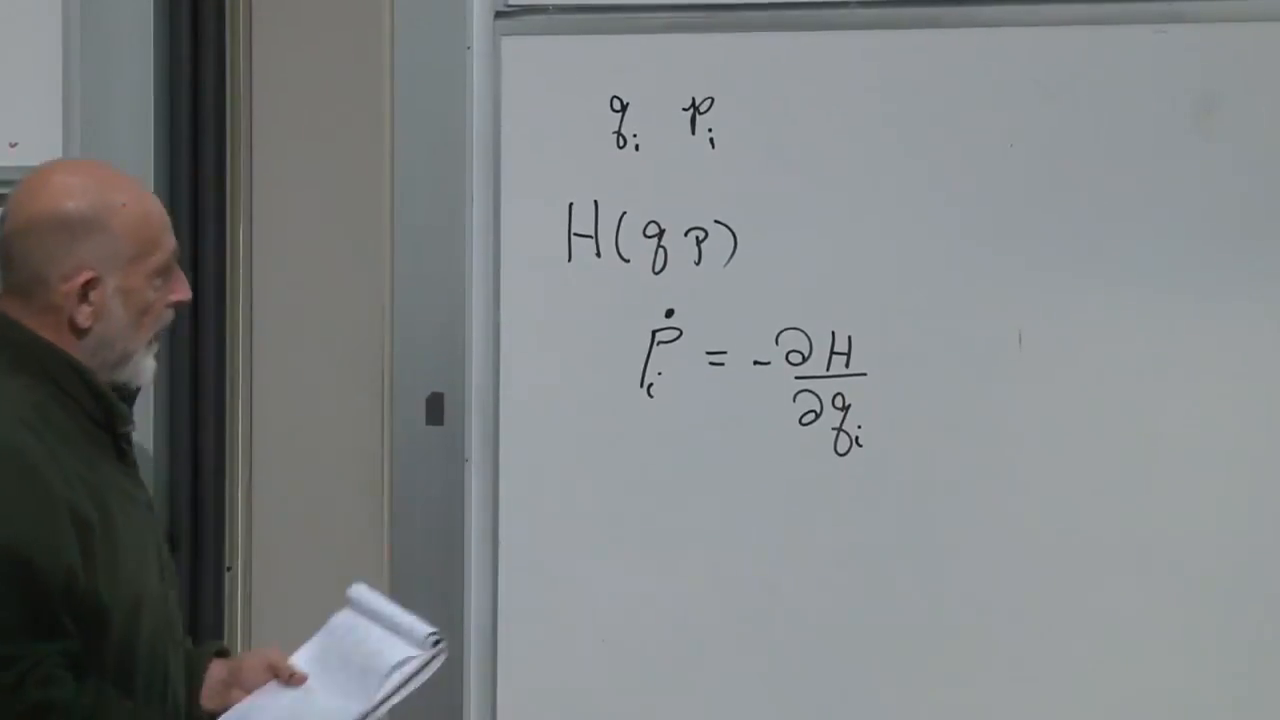
\includegraphics[width=0.82\textwidth]{lecture_07_figure_02.png}
  \caption{Канонические переменные, функция \(H(q,p)\) и гамильтоново уравнение для импульса в начале повторения.}
  \lectureframe{00:07:29}
\end{figure}

Хотя уравнения образуют пары с индексами, динамика вовсе не обязана разделяться по отдельным парам. Гамильтониан может связывать все \(q_i\) и \(p_i\), так что, например, \(\dot p_1\) может зависеть от состояния всей системы.

\begin{classroomqa}
  \audiencequestion{Является ли это изложение теперь аксиоматическим? Какое соотношение между \(p\) и \(q\) было предположено?
  \lecturetimestamp{00:17:08--00:18:18}}
  \lecturerresponse{Уравнения Гамильтона определяют формальную теорию, как только заданы \(H(q,p)\) и канонические пары. Никакого универсального дополнительного предположения \(p=m\dot q\) нет. Это соотношение выполняется для обычной частицы в декартовых координатах с квадратичной кинетической энергией, но другие координаты и другие гамильтонианы дают другие импульс--скоростные соотношения. Сами уравнения задают это соотношение через
  \(\dot q_i=\partial H/\partial p_i\). Реализуется ли предлагаемый гамильтониан в природе — отдельный физический вопрос.}
\end{classroomqa}

Теперь мы можем восстановить сохранение энергии одним рассуждением. Вдоль траектории полная производная \(H\) равна
\begin{equation}
  \frac{dH}{dt}
  =
  \sum_i\left(
    \frac{\partial H}{\partial q_i}\dot q_i
    +\frac{\partial H}{\partial p_i}\dot p_i
  \right)
  +\frac{\partial H}{\partial t}.
  \label{eq:l7-total-h-derivative}
\end{equation}
Последний член означает явную зависимость от времени при фиксированных \(q\) и \(p\), возможно потому, что меняется внешне заданный параметр. Подставляя уравнение~\eqref{eq:l7-hamilton-equations},
\begin{align}
  \frac{dH}{dt}
  &=
  \sum_i\left[
    \frac{\partial H}{\partial q_i}
    \frac{\partial H}{\partial p_i}
    -\frac{\partial H}{\partial p_i}
    \frac{\partial H}{\partial q_i}
  \right]
  +\frac{\partial H}{\partial t}\\
  &=\frac{\partial H}{\partial t}.
  \label{eq:l7-h-energy-rate}
\end{align}
Каждый член в сумме сокращается со своим парным членом. Следовательно,
\begin{equation}
  \frac{\partial H}{\partial t}=0
  \quad\Longrightarrow\quad
  \frac{dH}{dt}=0.
  \label{eq:l7-energy-conservation}
\end{equation}
Для замкнутой системы, инвариантной относительно сдвигов по времени, гамильтониан сохраняется и является энергией.

\begin{classroomqa}
  \audiencequestion{Что меняется, если гамильтониан явно зависит от времени?
  \lecturetimestamp{00:10:32--00:12:33}}
  \lecturerresponse{Тогда уравнение~\eqref{eq:l7-h-energy-rate} по-прежнему выполняется, но энергия подсистемы не обязана быть постоянной. Явная зависимость от времени обычно представляет неучтенный внешний привод, обменивающийся энергией с системой. Если этот привод включить как динамическую часть более крупной замкнутой системы, больший гамильтониан снова может не зависеть от времени явно, и его полная энергия сохраняется.}
\end{classroomqa}

\section{Энергия как геометрия в фазовом пространстве}

Предположим теперь, что \(H\) не имеет явной зависимости от времени. Начальное условие фиксирует число \(E\), и фазовая точка остается на
\begin{equation}
  H(q,p)=E.
  \label{eq:l7-energy-surface}
\end{equation}
Фазовое пространство имеет \(2n\) измерений. В регулярных точках одно уравнение на его координаты задает \((2n-1)\)-мерную гиперповерхность. Разные значения \(E\) дают разные гиперповерхности. Они не обязаны быть замкнутыми или компактными; сохранение энергии утверждает лишь, что траектория, начинающаяся на одной из них, никогда ее не покидает.

Для приведенного гармонического осциллятора из предыдущей лекции,
\begin{equation}
  H=\frac{\omega}{2}(p^2+q^2).
  \label{eq:l7-oscillator-hamiltonian}
\end{equation}
Следовательно, каждое множество постоянной энергии есть окружность,
\begin{equation}
  p^2+q^2=\frac{2E}{\omega}.
  \label{eq:l7-oscillator-circle}
\end{equation}

\begin{figure}[htbp]
  \centering
  \includegraphics[width=0.84\textwidth]{lecture_07_figure_04.png}
  \caption{Схема \(2n\)-мерного фазового пространства и гамильтониан гармонического осциллятора, используемые для введения поверхностей постоянной энергии.}
  \lectureframe{00:15:20}
\end{figure}

Уравнения движения,
\begin{equation}
  \dot q=\omega p,\qquad \dot p=-\omega q,
  \label{eq:l7-oscillator-flow}
\end{equation}
задают движение точки по часовой стрелке вдоль своей окружности. Уравнение энергии говорит, какая кривая содержит движение; уравнения Гамильтона задают направление и скорость вдоль этой кривой.

\begin{figure}[htbp]
  \centering
  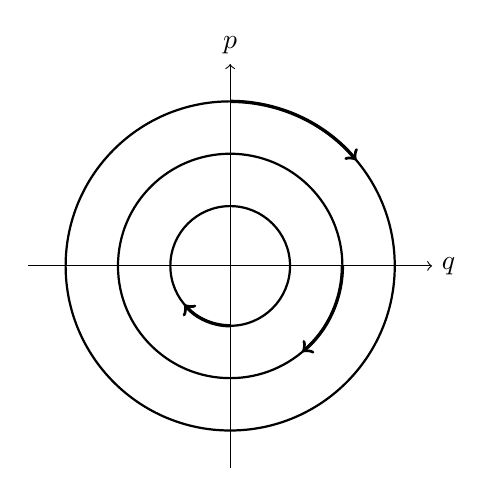
\begin{tikzpicture}[scale=0.95]
    \draw[->] (-2.7,0) -- (2.7,0) node[right] {\(q\)};
    \draw[->] (0,-2.7) -- (0,2.7) node[above] {\(p\)};
    \draw[thick] (0,0) circle (0.8);
    \draw[thick] (0,0) circle (1.5);
    \draw[thick] (0,0) circle (2.2);
    \draw[->,very thick] (0,2.2) arc[start angle=90,end angle=40,radius=2.2];
    \draw[->,very thick] (1.5,0) arc[start angle=0,end angle=-50,radius=1.5];
    \draw[->,very thick] (0,-0.8) arc[start angle=-90,end angle=-140,radius=0.8];
  \end{tikzpicture}
  \caption{Постоянная энергия задает окружности; уравнения осциллятора задают касательный поток по часовой стрелке.}
\end{figure}

\begin{classroomqa}
  \audiencequestion{Являются ли два уравнения Гамильтона и \(H=E\) несколькими версиями одного и того же уравнения?
  \lecturetimestamp{00:15:53--00:17:06}}
  \lecturerresponse{Нет. Уравнения Гамильтона — это два закона движения первого порядка для одной канонической пары. Они влекут \(dH/dt=0\), из которого следует \(H=E\). Значение \(E\) выбирается начальным условием. Уравнение \(H=E\) задает поверхность; само по себе оно не определяет скорость вдоль этой поверхности.}
\end{classroomqa}

\section{От одного состояния к потоку состояний}

Вместо того чтобы следить за одним начальным условием, рассыпьте по фазовому пространству все возможные начальные условия и запустите часы. Каждая точка — это полное возможное состояние, и каждое состояние движется согласно уравнениям Гамильтона. Это рассеяние можно вообразить как пыль или как воображаемую жидкость. Ничего материального в фазовое пространство не наливают; жидкость — это способ увидеть все траектории сразу.

Поле скоростей в фазовом пространстве имеет вид
\begin{equation}
  \mathbf V(q,p,t)
  =
  (\dot q_1,\ldots,\dot q_n,\dot p_1,\ldots,\dot p_n).
  \label{eq:l7-phase-velocity}
\end{equation}
Для одной канонической пары пишем
\begin{equation}
  V_q=\dot q=\frac{\partial H}{\partial p},
  \qquad
  V_p=\dot p=-\frac{\partial H}{\partial q}.
  \label{eq:l7-phase-components}
\end{equation}
В каждой точке гамильтониан задает вектор, указывающий фазовой точке, куда идти дальше. Если \(H\) не зависит от времени, векторное поле стационарно: возвращение в ту же фазовую точку дает ту же скорость. Если \(H\) зависит от времени, само векторное поле меняется со временем, но в каждый момент оно все равно определено.

\begin{figure}[htbp]
  \centering
  \includegraphics[width=0.84\textwidth]{lecture_07_figure_05.png}
  \caption{Поле скоростей гармонического осциллятора. Векторы касательны к окружностям и укорачиваются по мере приближения к началу координат.}
  \lectureframe{00:24:50}
\end{figure}

Для гармонического осциллятора каждый радиус-вектор вращается с угловой скоростью \(\omega\). Точки вблизи начала координат имеют меньшую линейную скорость, потому что за тот же период проходят окружность меньшей длины. Поэтому вся пыль вращается как жесткая карусель.

\begin{classroomqa}
  \audiencequestion{Означает ли жесткое вращение, что все траектории осциллятора имеют один и тот же период? \lecturetimestamp{00:21:10--00:21:42}}
  \lecturerresponse{Да. Именно эта независимость от амплитуды и есть определяющее особое свойство гармонического осциллятора. Каждая окружность обходится с одной и той же угловой частотой \(\omega\), хотя модуль скорости в фазовом пространстве на меньшей окружности меньше.}
\end{classroomqa}

\begin{classroomqa}
  \audiencequestion{Одинаков ли вектор скорости в фазовом пространстве в каждой точке?
  \lecturetimestamp{00:24:29--00:25:37}}
  \lecturerresponse{Нет. И его направление, и его модуль в общем случае зависят от положения. Для осциллятора этот вектор касается локальной окружности и имеет модуль \(\omega\sqrt{p^2+q^2}\). Векторное поле означает, что каждой точке поставлен в соответствие один вектор, а не что повсюду скопирован один и тот же вектор.}
\end{classroomqa}

\begin{classroomqa}
  \audiencequestion{Что именно здесь играет роль частиц и плотности этой воображаемой жидкости? \lecturetimestamp{00:56:03--00:58:40}}
  \lecturerresponse{Каждая точка — это одно полное состояние всей механической системы. Это не отдельная физическая частица. Для пяти частиц, движущихся в одном пространственном измерении, нужны пять координат и пять импульсов, следовательно, фазовое пространство 10-мерно; в трех измерениях требуется 30 измерений. Эта пыль есть ансамбль альтернативных состояний. Если образ жидкости отвлекает, просто возьмите область начальных условий, проследите эволюцию каждой точки в ней и сравните ее объем в фазовом пространстве до и после.}
\end{classroomqa}

\section{Сжатие и дивергенция}

Чтобы выяснить, теряет ли эта воображаемая жидкость объем, начнем с одного измерения.
Пусть точки на прямой движутся со скоростью \(v(x)\). Для двух близких точек, разделенных расстоянием \(\delta x\), разность скоростей равна
\begin{equation}
  \delta v \simeq \frac{dv}{dx}\,\delta x.
  \label{eq:l7-one-dimensional-strain}
\end{equation}
Если \(dv/dx>0\), передняя точка движется быстрее, и интервал растягивается. Если
\(dv/dx<0\), он сжимается. Стационарное одномерное несжимаемое течение,
следовательно, удовлетворяет
\begin{equation}
  \frac{dv}{dx}=0.
  \label{eq:l7-one-dimensional-incompressible}
\end{equation}

\begin{figure}[htbp]
  \centering
  \includegraphics[width=0.84\textwidth]{lecture_07_figure_06.png}
  \caption{Одномерная конструкция, приводящая к \(dv/dx\) как к локальной скорости растяжения или сжатия.}
  \lectureframe{00:30:20}
\end{figure}

Есть две эквивалентные точки зрения. Мы можем следить за материальным отрезком и спрашивать, меняется ли его длина. Или можем удерживать малый отрезок фиксированным и спрашивать, равно ли количество, входящее за единицу времени, количеству, выходящему.
В первом случае мы следуем за жидкостью; во втором наблюдаем, как она проходит мимо.

В размерности больше единицы область может растягиваться вдоль одной оси и сжиматься вдоль другой, не меняя полного объема. Для поля скоростей
\(\mathbf V=(V_x,V_y,V_z)\), соответствующей локальной величиной является дивергенция,
\begin{equation}
  \nabla\cdot\mathbf V
  =
  \frac{\partial V_x}{\partial x}
  +\frac{\partial V_y}{\partial y}
  +\frac{\partial V_z}{\partial z}.
  \label{eq:l7-spatial-divergence}
\end{equation}
Положительная дивергенция означает локальное расширение, отрицательная — локальное
сжатие, а несжимаемость выражается условием
\begin{equation}
  \nabla\cdot\mathbf V=0.
  \label{eq:l7-zero-divergence}
\end{equation}
Равенство притока и оттока через фиксированный малый ящик — это то же локальное утверждение,
что и сохранение объема малого ящика, движущегося вместе с потоком.

\begin{figure}[htbp]
  \centering
  \includegraphics[width=0.86\textwidth]{lecture_07_figure_07.png}
  \caption{Двумерный ящик, его компоненты потока и сумма производных по соответствующим координатам, определяющая дивергенцию.}
  \lectureframe{00:35:30}
\end{figure}

\begin{classroomqa}
  \audiencequestion{Идет ли речь о жидкости в обычном пространстве или о потоке в
  фазовом пространстве? \lecturetimestamp{00:34:27--00:34:40}}
  \lecturerresponse{Сначала это просто общее рассуждение о жидкости.
  Мы применим его к фазовому пространству четной размерности, где координатными
  направлениями являются \(q_i\) и \(p_i\), а компонентами скорости —
  \(\dot q_i\) и \(\dot p_i\).}
\end{classroomqa}

Теперь вернемся к дискретным отображениям состояний. В обратимом цикле в каждый узел
входит одна стрелка и из него выходит одна стрелка, и выбранное множество состояний сохраняет
то же число элементов по мере эволюции. В стоке входит много стрелок, а выходит слишком мало;
несколько альтернатив становятся неразличимыми.

\begin{figure}[htbp]
  \centering
  \includegraphics[width=0.80\textwidth]{lecture_07_figure_08.png}
  \caption{Дискретный сток, используемый, чтобы вновь связать дивергенцию с
  критерием обратимых законов из первой лекции.}
  \lectureframe{00:40:15}
\end{figure}

Теперь в непрерывном случае вопрос ставится точно: имеет ли гамильтонов поток нулевую
дивергенцию, так что малая область различимых состояний никогда не сплющивается в меньший
объем фазового пространства?

\section{Теорема Лиувилля}

\begin{theorem}[Liouville's theorem]
Для гладкой гамильтоновой системы каноническое поле скоростей в фазовом пространстве имеет
нулевую дивергенцию:
\begin{equation}
  \sum_i\left(
    \frac{\partial\dot q_i}{\partial q_i}
    +\frac{\partial\dot p_i}{\partial p_i}
  \right)=0.
  \label{eq:l7-liouville-divergence}
\end{equation}
Эквивалентно, гамильтонова эволюция сохраняет канонический фазовый объем
\(dq_1\cdots dq_n\,dp_1\cdots dp_n\).
\end{theorem}

\begin{classroomqa}
  \audiencequestion{Компоненты, обозначенные \(V\), — это просто производные по времени от \(p\) и
  \(q\)? \lecturetimestamp{00:42:20--00:43:22}}
  \lecturerresponse{Да. Для одной пары
  \(V_q=\dot q\) и \(V_p=\dot p\). Если выписать все такие производные в ряд, получится
  вектор скорости потока во всем фазовом пространстве.}
\end{classroomqa}

Для одной канонической пары уравнения Гамильтона дают
\begin{equation}
  V_p=-\frac{\partial H}{\partial q},
  \qquad
  V_q=\frac{\partial H}{\partial p}.
  \label{eq:l7-liouville-components}
\end{equation}
Поэтому дивергенция равна
\begin{align}
  \frac{\partial V_p}{\partial p}
  +\frac{\partial V_q}{\partial q}
  &=
  -\frac{\partial}{\partial p}
    \left(\frac{\partial H}{\partial q}\right)
  +\frac{\partial}{\partial q}
    \left(\frac{\partial H}{\partial p}\right)\\
  &=
  -\frac{\partial^2H}{\partial p\,\partial q}
  +\frac{\partial^2H}{\partial q\,\partial p}
  =0.
  \label{eq:l7-liouville-proof}
\end{align}

\begin{figure}[htbp]
  \centering
  \includegraphics[width=0.86\textwidth]{lecture_07_figure_09.png}
  \caption{Прямоугольник конечных разностей, используемый для объяснения того, почему гладкие смешанные
  частные производные перестановочны.}
  \lectureframe{00:47:30}
\end{figure}

Равенство смешанных частных производных можно увидеть, если рассмотреть четыре близкие точки
\(A,B,C,D\) в вершинах малого прямоугольника в плоскости \(q\)-\(p\).
Сначала взяв разность по \(q\), а затем по \(p\), мы получаем, с точностью до множителя из двух
малых длин сторон,
\begin{equation}
  F(B)+F(D)-F(A)-F(C).
  \label{eq:l7-finite-difference-combination}
\end{equation}
Если брать разности в обратном порядке, получается та же комбинация.
В пределе малого прямоугольника это дает
\(\partial_p\partial_qF=\partial_q\partial_pF\), при условии непрерывности требуемых
производных.

\begin{figure}[htbp]
  \centering
  \includegraphics[width=0.88\textwidth]{lecture_07_figure_10.png}
  \caption{Каноническая дивергенция после того, как уравнения Гамильтона свели
  ее к двум смешанным производным с противоположными знаками.}
  \lectureframe{00:50:20}
\end{figure}

Для многих степеней свободы то же сокращение происходит для каждой канонической
пары:
\begin{align}
  \sum_i\left(
    \frac{\partial\dot p_i}{\partial p_i}
    +\frac{\partial\dot q_i}{\partial q_i}
  \right)
  &=
  \sum_i\left(
    -\frac{\partial^2H}{\partial p_i\,\partial q_i}
    +\frac{\partial^2H}{\partial q_i\,\partial p_i}
  \right)\\
  &=0.
  \label{eq:l7-many-pair-proof}
\end{align}
Растяжение вдоль одного канонического направления уравновешивается сжатием в его
сопряженном направлении. Такое попарное сокращение выражает более сильную структуру, чем
случайная компенсация между несвязанными осями.

\begin{classroomqa}
  \audiencequestion{Подразумевается ли суммирование по всем каноническим парам?
  \lecturetimestamp{00:52:00--00:52:36}}
  \lecturerresponse{Да. В формуле~\eqref{eq:l7-many-pair-proof} суммирование ведется по
  \(i\), и две смешанные производные сокращаются отдельно внутри каждой
  пары \(q_i,p_i\).}
\end{classroomqa}

\begin{classroomqa}
  \audiencequestion{Выписанная дивергенция выглядит декартовой. Сохраняется ли
  теорема при замене координат?
  \lecturetimestamp{00:52:50--00:53:22,\allowbreak\ 00:58:18--00:58:40}}
  \lecturerresponse{Естественная формулировка дается в канонических координатах
  и с каноническим элементом объема
  \(dq_1\cdots dq_n\,dp_1\cdots dp_n\). Каноническое, или симплектическое,
  преобразование совместно изменяет координаты и импульсы и сохраняет этот
  объем. В произвольных неканонических координатах в мере объема должен
  присутствовать якобиан; наивное произведение приращений координат не обязано
  быть инвариантным.}
\end{classroomqa}

\begin{classroomqa}
  \audiencequestion{Требует ли теорема Лиувилля гамильтониана, не зависящего от
  времени? \lecturetimestamp{00:53:43--00:55:51}}
  \lecturerresponse{Нет. Сохранение энергии требовало
  \(\partial H/\partial t=0\), но доказательство для дивергенции дифференцирует только
  по \(q_i\) и \(p_i\) при фиксированном времени. Смешанные частные производные по-прежнему
  сокращаются для \(H(q,p,t)\). Следовательно, зависящий от времени гамильтониан
  порождает зависящий от времени, но в каждый данный момент сохраняющий объем
  канонический поток.}
\end{classroomqa}

\section{Что означает и чего не означает сохранение объема}

Возьмите любую малую область \(R_0\) начальных условий и проследите эволюцию каждой точки в течение
времени \(t\). Теорема Лиувилля утверждает
\begin{equation}
  \operatorname{Vol}(R_t)=\operatorname{Vol}(R_0).
  \label{eq:l7-volume-preservation}
\end{equation}
Область может перемещаться, вращаться, деформироваться сдвигом и вытягиваться в длинную нить. Ее
объем, а не форма, сохраняется. Различные фазовые точки не могут сливаться при
конечной гладкой гамильтоновой эволюции.

Для конечных времен гладкий гамильтонов поток представляет собой обратимое отображение с гладким
обратным отображением, получаемым эволюцией назад по времени. Это также объясняет прозвучавшее
на лекции утверждение, что связная область не может перетянуться и распасться на несвязанные части:
поток непрерывно деформирует область и сохраняет ее топологию, хотя чрезвычайно тонкая перемычка
может при конечном разрешении создать видимость, что две доли разделены.

\begin{figure}[htbp]
  \centering
  \includegraphics[width=0.86\textwidth]{lecture_07_figure_12.png}
  \caption{Возможные деформации одной области фазового пространства. Гладкий
  гамильтонов поток может образовать тонкую перемычку, но не подлинный разрыв за конечное время
  на части, эволюционирующие независимо.}
  \lectureframe{01:04:55}
\end{figure}

\begin{classroomqa}
  \audiencequestion{Может ли область фазового пространства перетянуться и разделиться на две
  части? \lecturetimestamp{01:04:10--01:05:49}}
  \lecturerresponse{Не при гладком детерминистическом гамильтоновом потоке за
  конечное время. В гипотетической точке пережатия по-прежнему есть одна точка фазового пространства
  и одна приписанная ей скорость, а не два несовместимых направления. Область
  может образовать очень длинную узкую соединяющую нить, но
  эволюция остается взаимно однозначной и не разрывает ее.}
\end{classroomqa}

\begin{classroomqa}
\audiencequestion{Являются ли две далеко разошедшиеся части растянутого пятна физически связанными или квантово запутанными?
\lecturetimestamp{01:08:01--01:09:16}}
\lecturerresponse{Никакая такая физическая связь не подразумевается. Это пятно — набор альтернативных начальных условий, а не один материальный объект. Называя его одной областью, мы лишь фиксируем общее множество, из которого эволюционировали эти состояния; это ничего не говорит ни о силах между ними, ни о квантовой запутанности.
}
\end{classroomqa}

\begin{classroomqa}
\audiencequestion{Что происходит вблизи верхнего неустойчивого равновесия жёсткого маятника? Перекрываются ли траектории, идущие по часовой стрелке и против неё?
\lecturetimestamp{01:07:07--01:07:47}}
\lecturerresponse{Близкие начальные условия могут разойтись по очень разным траекториям, образуя только что описанные тонкие нити. Они не становятся одной и той же точкой фазового пространства: две стороны различаются знаком бесконечно малого смещения или импульса. Состояние точного баланса имеет собственное однозначно определённое движение, а именно в идеальной модели остаётся в равновесии.}
\end{classroomqa}

\subsection{Растяжение в пространстве координат и сжатие в пространстве импульсов}

Если каноническое преобразование растягивает некоторый диапазон координат в \(a\) раз,
то масштаб сопряжённого импульса сжимается в обратное число раз:
\begin{equation}
  q\longrightarrow aq,
  \qquad
  p\longrightarrow \frac{p}{a},
  \qquad
  dq\,dp\longrightarrow dq\,dp.
  \label{eq:l7-canonical-scaling}
\end{equation}
В этом состоит ясное фазово-пространственное содержание примера с расширением газа. При адиабатическом расширении доступная область обычного пространства увеличивается, тогда как типичные импульсы уменьшаются и газ охлаждается. Конкретное термодинамическое соотношение зависит от размерности, протокола расширения и взаимодействий; теорема Лиувилля задаёт ограничение на объём, а не каждый термодинамический коэффициент.

\begin{classroomqa}
\audiencequestion{Применимо ли то же рассуждение к расширяющейся Вселенной, даже при внезапном расширении? \lecturetimestamp{00:53:23--00:56:00}}
\lecturerresponse{Теорема Лиувилля применима всякий раз, когда полная динамика является гамильтоновой, включая случай явно зависящих от времени канонических переменных. Расширение по координатным направлениям должно сопровождаться соответствующим сжатием по направлениям канонических импульсов. Однако космологический масштабный фактор, управляемое расширение газа и свободно разлетающееся облако — не один и тот же физический процесс. Хабблоподобная корреляция между расстоянием и скоростью удаления может возникать потому, что более быстрые объекты улетают дальше, тогда как адиабатическое охлаждение связано со сжатием локального распределения импульсов. В обоих случаях теорема накладывает ограничение на полное отображение фазового пространства.}
\end{classroomqa}

\begin{classroomqa}
\audiencequestion{Какое практическое применение имеет теорема Лиувилля?
\lecturetimestamp{01:06:16--01:07:04}}
\lecturerresponse{Она занимает центральное место в статистической механике. Она определяет, как эволюционируют ансамбли микроскопических состояний, и лежит в основе связи между объёмом фазового пространства и энтропией. Расширение и охлаждение газа — одна непосредственная иллюстрация; далее она становится базовым инструментом для рассуждений о равновесных и неравновесных системах.}
\end{classroomqa}

\section{Поток, резко меняющий форму}

Гармонический осциллятор сохраняет и площадь, и форму, потому что его поток представляет собой жёсткое вращение. Это исключительный случай. Чтобы отделить сохранение объёма от жёсткости, рассмотрим
\begin{equation}
  H=\lambda pq,
  \label{eq:l7-pq-hamiltonian}
\end{equation}
где \(\lambda\) имеет размерность обратного времени. В лекции полагается
\(\lambda=1\); сохраняя этот параметр, мы явно видим размерности.

\begin{figure}[htbp]
\centering
  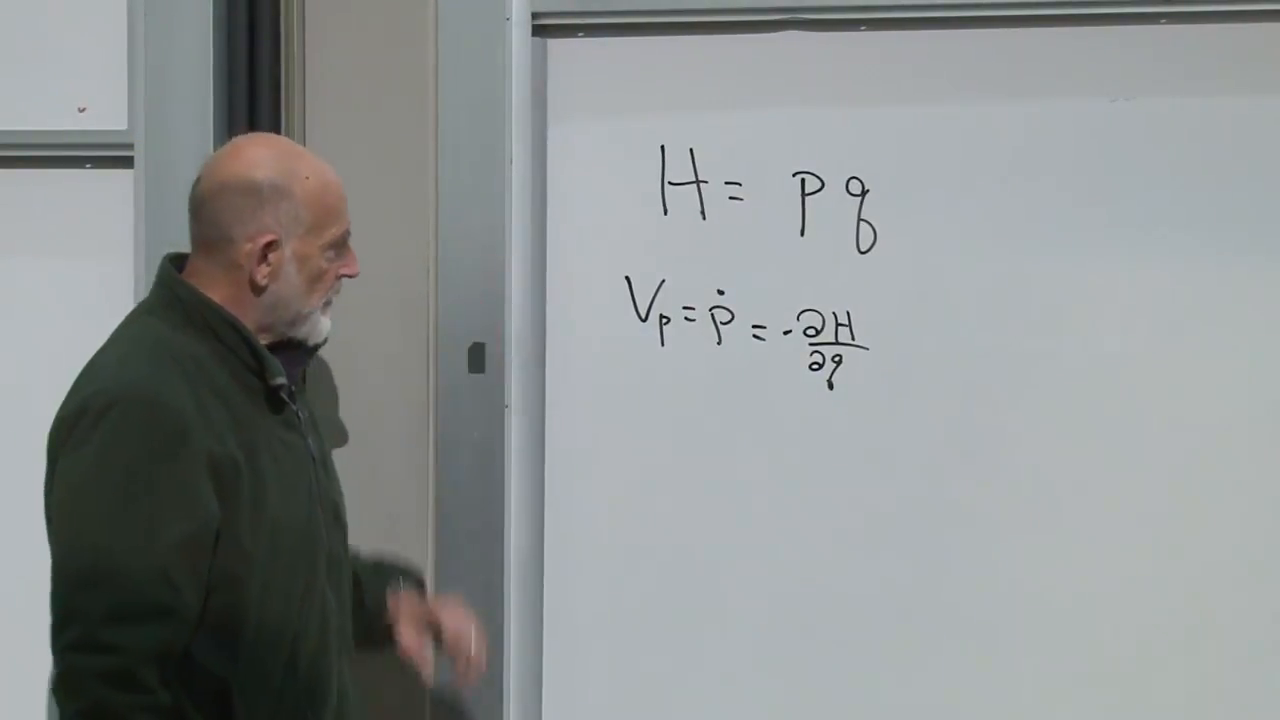
\includegraphics[width=0.82\textwidth]{lecture_07_figure_03.png}
\caption{Начало примера с \(H=pq\) и первая компонента фазовой скорости.}
\lectureframe{01:00:11}
\end{figure}

Уравнения Гамильтона имеют вид
\begin{equation}
  \dot p=-\lambda p,
  \qquad
  \dot q=\lambda q,
  \label{eq:l7-pq-flow}
\end{equation}
с решениями
\begin{equation}
  p(t)=p_0e^{-\lambda t},
  \qquad
  q(t)=q_0e^{\lambda t}.
  \label{eq:l7-pq-solutions}
\end{equation}
Квадратный участок экспоненциально сжимается по \(p\) и растягивается на тот же множитель по \(q\):
\begin{equation}
  \Delta p(t)\Delta q(t)
  =
  \Delta p(0)\Delta q(0).
  \label{eq:l7-pq-area}
\end{equation}
Дивергенция потока локально подтверждает этот результат,
\begin{equation}
  \frac{\partial\dot p}{\partial p}
  +\frac{\partial\dot q}{\partial q}
  =-\lambda+\lambda=0.
  \label{eq:l7-pq-divergence}
\end{equation}

\begin{figure}[htbp]
\centering
  \includegraphics[width=0.86\textwidth]{lecture_07_figure_11.png}
\caption{Компактный участок, растянутый в длинную тонкую полосу при сохранении площади в потоке \(H=pq\).}
\lectureframe{01:02:10}
\end{figure}

\begin{classroomqa}
\audiencequestion{Поскольку \(pq\) имеет размерность действия, является ли теорема Лиувилля законом сохранения действия? \lecturetimestamp{01:03:00--01:04:09}}
\lecturerresponse{Нет. Теорема сохраняет объём фазового пространства. Для одной канонической пары \(dq\,dp\) имеет размерность действия, и этот факт размерности предвосхищает квантовую механику, где ячейки фазового пространства измеряются в единицах, задаваемых \(\hbar\). Но произведение \(pq\) само по себе не является функционалом действия Гамильтона и не становится автоматически моментом импульса лишь потому, что размерности совпадают.}
\end{classroomqa}

Этот пример также показывает, что углы не обязаны сохраняться. Прямоугольный крест с неравными компонентами при масштабировании по формуле~\eqref{eq:l7-pq-solutions} как метрическая фигура подвергается сдвиговой деформации, тогда как площадь остаётся неизменной. Теорема Лиувилля — это теорема о площади или объёме, а не обычная теорема об евклидовой жёсткости.

\section{Затухание порождает сток}

Чтобы увидеть, что именно исключает теорема, рассмотрим редуцированное уравнение для затухающего осциллятора,
\begin{equation}
  m\ddot x=-kx-c\dot x,
  \qquad c>0.
  \label{eq:l7-damped-newton}
\end{equation}
Положим \(p=m\dot x\). Тогда
\begin{equation}
  \dot x=\frac{p}{m},
  \qquad
  \dot p=-kx-\frac{c}{m}p.
  \label{eq:l7-damped-first-order}
\end{equation}
Без затухания фазовая точка обращается вокруг начала координат. При наличии затухания энергия передаётся микроскопическим степеням свободы окружающей среды, и орбита закручивается внутрь по спирали.

\begin{figure}[htbp]
\centering
  \includegraphics[width=0.84\textwidth]{lecture_07_figure_13.png}
\caption{Уравнение затухающего осциллятора и его спираль, закручивающаяся внутрь, на плоскости \(x\)-\(p\).}
\lectureframe{01:13:30}
\end{figure}

Дивергенция этого редуцированного двумерного потока равна
\begin{equation}
  \frac{\partial\dot x}{\partial x}
  +\frac{\partial\dot p}{\partial p}
  =
  0-\frac{c}{m}<0.
  \label{eq:l7-damped-divergence}
\end{equation}
Любой конечный участок сжимается. Начало координат является стоком, непрерывным аналогом диаграммы состояний, в которой многие стрелки входят в одно состояние.

\begin{figure}[htbp]
\centering
  \includegraphics[width=0.88\textwidth]{lecture_07_figure_14.png}
\caption{Компоненты фазовой скорости при затухании, использованные для получения отрицательной дивергенции \(-c/m\).}
\lectureframe{01:16:05}
\end{figure}

Это не означает, что микроскопическая механика нарушает теорему Лиувилля. Две переменные \(x,p\) не учитывают огромное число степеней свободы среды, которые принимают энергию осциллятора. Расширенная система «осциллятор плюс среда» может быть гамильтоновой и сохранять объём, хотя её редуцированное описание в переменных \(x,p\) сжимается.

\begin{classroomqa}
\audiencequestion{Описывается ли затухающий осциллятор по-прежнему уравнением Ньютона, хотя в этом редуцированном фазовом пространстве он не является гамильтоновым?
\lecturetimestamp{01:20:09--01:21:12}}
\lecturerresponse{Да. В \(F=ma\) можно включить эмпирически заданную силу сопротивления. Элементарное описание с \(L=T-V\) и гамильтонианом непосредственно применимо к консервативным силам, а более общие лагранжианы позволяют учитывать и некоторые силы, зависящие от скорости. Однако марковский член трения для изолированной пары \(x,p\) — это редуцированная диссипативная динамика, а не замкнутая каноническая гамильтонова система.}
\end{classroomqa}

\begin{classroomqa}
\audiencequestion{Если затухающие уравнения можно интегрировать назад при бесконечной точности, действительно ли информация теряется?
\lecturetimestamp{01:25:16--01:27:17}}
\lecturerresponse{Для любого конечного времени идеальное дифференциальное уравнение всё ещё имеет обратное отображение, так что точные данные можно проследить назад. Точное утверждение состоит в том, что конечные ячейки фазового пространства экспоненциально сжимаются. Поэтому восстановление их прошлого требует экспоненциально растущей точности, а при бесконечном времени все траектории приближаются к стоку. Это наиболее близкий непрерывный классический аналог дискретной картины потери альтернатив, а не утверждение, будто два точных решения при конечном времени буквально становятся одним.}
\end{classroomqa}

\begin{classroomqa}
\audiencequestion{Может ли векторное поле иметь нулевую дивергенцию, не будучи порождённым гамильтонианом? \lecturetimestamp{01:18:21--01:22:34}}
\lecturerresponse{Конечно. Гамильтонова форма достаточна для нулевой дивергенции, но не необходима. Произвольное несжимаемое поле скоростей может иметь нулевую дивергенцию, не будучи каноническим гамильтоновым полем на том же самом пространстве. Обычный учебный пример — трёхмерное несжимаемое поле скорости жидкости: три координаты сами по себе не могут образовать канонические пары. Полная механика жидкости может допускать более сложные бесконечномерные гамильтоновы формулировки, но это не отменяет одностороннего следствия, о котором здесь идёт речь.}
\end{classroomqa}

\section{Дополнительные различия, выявленные вопросами}

\begin{classroomqa}
\audiencequestion{Как связано движение по поверхности постоянной энергии с сохранением всего объёма фазового пространства?
\lecturetimestamp{01:28:47--01:30:41}}
\lecturerresponse{Это независимые следствия гамильтоновой структуры. Если \(H\) не зависит от времени, каждая траектория остаётся на своей собственной поверхности энергии. Конечный участок может пересекать много таких поверхностей; теорема Лиувилля утверждает, что объём всего этого участка сохраняется. Для гармонического осциллятора этот участок сохраняет также и форму, потому что поток представляет собой жёсткое вращение. Для \(H=pq\) он сохраняет только площадь, но не форму.}
\end{classroomqa}

\begin{classroomqa}
  \audiencequestion{Как механическая работа вписывается в гамильтоново описание?
  \lecturetimestamp{01:30:44--01:32:57}}
  \lecturerresponse{Работа описывает энергию, передаваемую через выбранную границу системы. Внешний агент может поднять груз или изменить параметр и тем самым изменить энергию подсистемы; энергия, которую он сообщает, теряется самим агентом. Если обе стороны включены в одну замкнутую модель, акцент вновь смещается на сохранение полной энергии и обмен между подсистемами.}
\end{classroomqa}

\begin{classroomqa}
  \audiencequestion{Сохраняются ли при сохранении объема также топология и углы?
  \lecturetimestamp{01:33:00--01:33:37}}
  \lecturerresponse{Гладкий гамильтонов поток за конечное время сохраняет топологию, потому что он является обратимой непрерывной деформацией. В общем случае он не сохраняет евклидовы углы или форму. Жесткое вращение осциллятора их сохраняет, но растяжение при \(H=pq\) показывает, почему это особый случай.}
\end{classroomqa}

\begin{classroomqa}
  \audiencequestion{Было ли преобразование Лежандра опущено потому, что оно не имеет физического значения?
  \lecturetimestamp{01:33:43--01:34:48}}
  \lecturerresponse{Нет. Это полезное преобразование, которое заменяет описание через скорости описанием через импульсы и дает \(H=\sum_i p_i\dot q_i-L\), когда отображение регулярно. Эта конструкция уже неоднократно использовалась, даже когда ее формальное название не подчеркивалось; подробная общая теория просто не нужна для настоящей теоремы.}
\end{classroomqa}

\section{Скобки Пуассона: следующее сжатие}

В заключительные минуты изложение возвращается к исторической теме. Механика XIX века вновь и вновь искала компактные структуры, связывающие кажущиеся различными системы --- механику и геометрическую оптику, частицы и лучи, классические траектории и волновые описания. Скобки Пуассона — еще одна такая структура, и в квантовой механике они становятся особенно важными.

Пусть \(F(q,p)\) — любая функция на фазовом пространстве. Это может быть координата, импульс, произведение \(qp\) или момент импульса. В ходе движения имеем
\begin{equation}
  \frac{dF}{dt}
  =
  \sum_i\left(
    \frac{\partial F}{\partial q_i}\dot q_i
    +\frac{\partial F}{\partial p_i}\dot p_i
  \right).
  \label{eq:l7-f-time-derivative}
\end{equation}
Подставляя уравнения Гамильтона, получаем:
\begin{equation}
  \frac{dF}{dt}
  =
  \sum_i\left(
    \frac{\partial F}{\partial q_i}
    \frac{\partial H}{\partial p_i}
    -
    \frac{\partial F}{\partial p_i}
    \frac{\partial H}{\partial q_i}
  \right).
  \label{eq:l7-f-hamiltonian-derivative}
\end{equation}

\begin{figure}[htbp]
  \centering
  \includegraphics[width=0.88\textwidth]{lecture_07_figure_15.png}
  \caption{Правило цепочки для производной по времени от произвольной функции фазового пространства \(F(q,p)\).}
  \lectureframe{01:42:40}
\end{figure}

Повторяющаяся антисимметричная комбинация заслуживает названия. Для любых двух функций \(F\) и \(G\) определим их скобку Пуассона равенством
\begin{equation}
  \boxed{
  \{F,G\}
  =
  \sum_i\left(
    \frac{\partial F}{\partial q_i}
    \frac{\partial G}{\partial p_i}
    -
    \frac{\partial F}{\partial p_i}
    \frac{\partial G}{\partial q_i}
  \right).}
  \label{eq:l7-poisson-bracket}
\end{equation}

\begin{figure}[htbp]
  \centering
  \includegraphics[width=0.86\textwidth]{lecture_07_figure_16.png}
  \caption{Комбинация производных двух функций, получающая статус скобки Пуассона.}
  \lectureframe{01:44:15}
\end{figure}

Уравнение~\eqref{eq:l7-f-hamiltonian-derivative} принимает вид
\begin{equation}
  \boxed{\frac{dF}{dt}=\{F,H\}.}
  \label{eq:l7-hamiltonian-poisson-evolution}
\end{equation}
Если \(F\) также явно зависит от времени, следует добавить \(\partial F/\partial t\). При выборе \(F=q_i\) или \(F=p_i\) получаются два уравнения Гамильтона, так что уравнение~\eqref{eq:l7-hamiltonian-poisson-evolution} представляет собой компактную форму полной динамики.

Запись всегда можно искусственно сжать --- можно было бы возвести много уравнений в квадрат, сложить их и назвать результат одним уравнением. Это скорее скрывало бы структуру, чем выявляло ее. Скобка Пуассона полезна по противоположной причине: ее алгебра организует временную эволюцию, сохраняющиеся величины и симметрию. Следующий шаг — развить эту алгебру, а затем применить ее к моменту импульса, структура которого будет центральной и в классической механике, и в квантовой теории.

\section{Непрерывный смысл обратимости}

Теперь мы можем изложить эту цепочку идей, не сокращая ее. Уравнения Гамильтона сохраняют \(H\), когда гамильтониан не имеет явной зависимости от времени, так что отдельные траектории остаются на гиперповерхностях постоянной энергии. Те же уравнения задают скорость каждой точке фазового пространства. Дивергенция этой скорости обращается в нуль, поскольку смешанные частные производные попарно сокращаются. Следовательно, целая область возможных состояний сохраняет свой канонический объем.

Это непрерывная версия одной входящей и одной выходящей стрелки. Форма может изменяться, углы могут изменяться, и соседние траектории могут расходиться чрезвычайно сильно. Чего не может произойти в гладком замкнутом гамильтоновом описании, так это сжатия конечного набора альтернатив в меньший объем фазового пространства. Поток при \(H=pq\) демонстрирует возможность растяжения; редуцированный затухающий осциллятор демонстрирует сток, который появляется, как только от гамильтоновых условий отказываются. Скобки Пуассона затем сводят ту же динамику к утверждению, что гамильтониан порождает любую производную по времени.
